\chapter[SCP-155 无限速电脑]{
    SCP-155 Infinite Speed Computer \\
    SCP-155 无限速电脑
}

\label{chap:SCP-155}

\begin{figure}[H]
    \centering
    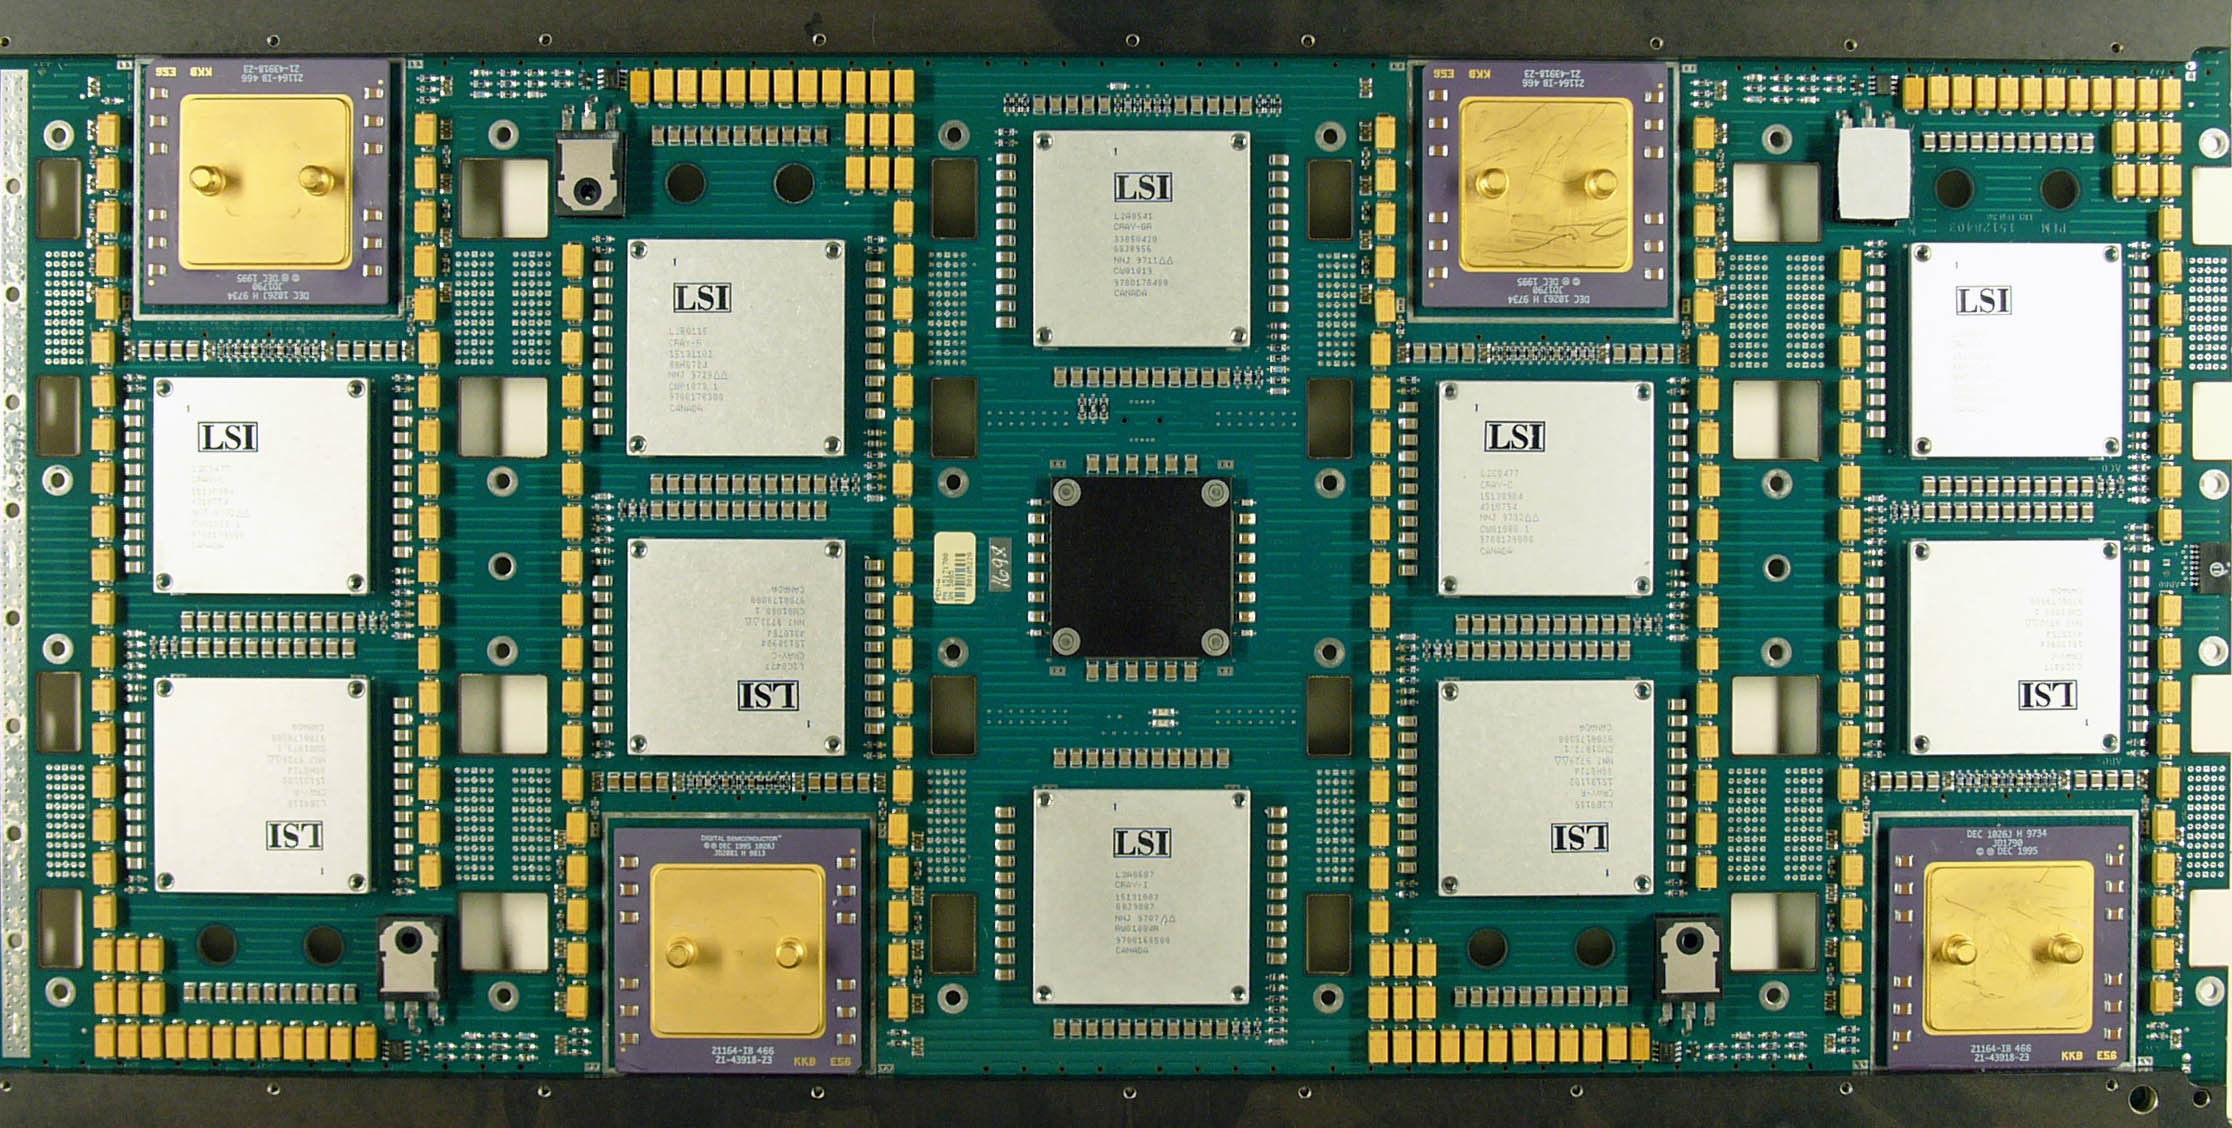
\includegraphics[width=0.5\linewidth]{images/SCP.155.jpg}
    \caption*{SCP-155上的一块非异常处理器板}
\end{figure}

\bb{项目编号:}SCP-155

\bb{项目等级:}Safe

\bb{特殊收容措施:}SCP-155将被收容于Site ██一隔热、防辐射收容间内。对SCP-155的回收文件和逆向工程汇总对所有有权限查看Site ██安保文件服务的人员开放,但在SCP-155上执行程序须由至少2名3级高级研究员事先批准。参见文件155-EXEC-1 以查看安全使用SCP-155所需的防辐射与隔热安保措施。\\
从事故155-08起,对SCP-155的试验已被全部推迟,直到SCP-155的前收容室被完全净化并将其转移到一个新收容室后。任何将要在SCP-155上运行的程序必须事先进行至少三次检查以确保其不会出现执行无法中止的情况。

\bb{描述:}SCP-155是一系列复杂电子设备,包括一台经由高度改装的Cray CS6400超级电脑、一台附属放射性同位素热电发电机和一台尚未被完全逆向解析的仪器。SCP-155是由机动特遣队Mu-4 ("Debuggers") 的队员在对毁灭后的普罗米修斯实验室设施进行搜查时从其主研究实验室中回收。

当程序和相关数据被录入SCP-155并被执行时,SCP-155会产生出一个半径5m的球形时间异常区。在该区域内的时间流速大幅加快,使得SCP-155的有效处理能力呈双曲线函数提高。一开始的程序执行速度十分缓慢,因为SCP-155的运行硬件十分老旧;但在保持运行8分14秒后SCP-155的有效处理速度将加速到趋向无限。从回收自普罗米修斯实验室的文件残篇来看, SCP-155曾被用于处理需要大量计算的任务,并能在数月内完成常规计算机需要数年才能完成的工作。

除了此种异常能力外,使用SCP-155有着极高的危险性:在程序执行期间SCP-155产生出的辐射和热能将聚集堆积,形成一个能量的“视界线”并在运行结束时释放。一个程序运行6分钟所产生的辐射量足以使得SCP-155收容室必须进过严格净化后才能允许让研究人员进入。

\bb{附录155-01:}事故155-08

于█\slash ██\slash ██, Dr. ███████ 将一个带有瑕疵的程序载入了SCP-155并导致其发生不可中止的执行(无限循环)。在研究员和技术人员发现该故障后,SCP-155被紧急关停,但直到8分3秒后才完全停止工作。此时,一阵强烈的热能和辐射波熔穿了SCP-155的收容间,最终导致了11人死亡并彻底破坏了Site██的C收容翼。SCP-155在事故中仅受到了极小的损伤,但相关实验已被推迟,正在审核经修订的安保措施并更换因过度加速时间出现老化的零件。
